\documentclass[10pt,a4paper]{article}
\usepackage[utf8]{inputenc}
\usepackage{amsmath}
\usepackage{amsfonts}
\usepackage{amssymb}
\usepackage{graphicx}
\usepackage{subfigure}
\usepackage{amsmath}
\usepackage{mathrsfs}
\DeclareRobustCommand{\orderof}{\ensuremath{\mathcal{O}}}
\bibliographystyle{prsty}
\usepackage[top=1in, bottom=1in, left=1in, right=1in]{geometry}

\begin{document}
\section{Introduction}
\textbf{dsa} is a task of application level. It can draw the density of state as a function of energy. Since the output data would be very large, only parts of the output data are attached. 

\section{Dictionary}

\subsection{Input}
\textit{\textbf{dsa.Mesh}} This parameter tells PiLab how to mesh the k-space. Input three integer values to tell PiLab how many divisions of each reciprocal vector. Since this task uses directly diagonalization rather than Green's function method to calculate the density of state, k-mesh should not be too sparse. It is suggested to have at least 200 k-points in total. \\ \\
\textit{\textbf{dsa.Interval}} This parameter sets the energy interval to count the number of states. If this parameter is too small, there will be a lot of delta functions in the spectrum. If it is too large, the spectrum may not reflect detail characteristics. So one should try and error to search for appropriate value. \\ \\
\textit{\textbf{dsa.Draw}} This parameter tells PiLab whether to draw the DOS spectrum or not. 'on'(default) or 'off. \\ \\
\textit{\textbf{dsa.Shift}} This parameter tells PiLab whether to shift Fermi level to zero. 'on'(default) or 'off'. Note that this is just to shift the plot. The original data will not change.


\subsection{Output}
\textit{\textbf{dsa.E\_dsa}} This variable outputs the number of states in a particular energy interval. First column is the energy and second is the number of states. Note that the number of density will be normalized to make the maximal value equal to 1.  


\begin{figure}[tbp]
\centering
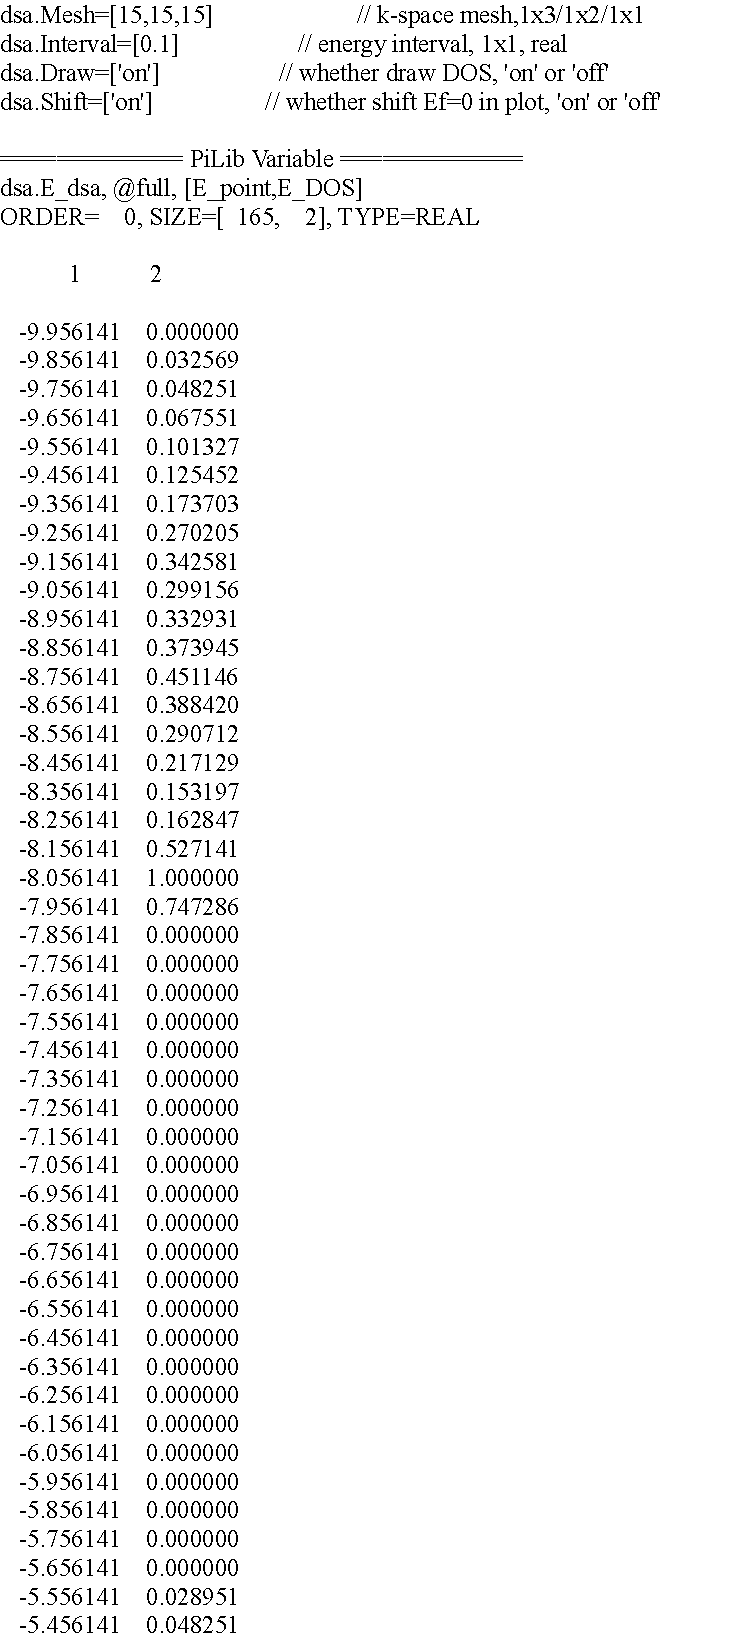
\includegraphics[width=0.9\columnwidth]{NiO_dsa.pdf}
\caption{NiO\_dsa.plb}
\end{figure}

\end{document}